\documentclass[aspectratio=1610,onlymath]{beamer}
% \documentclass[aspectratio=1610,onlymath,handout]{beamer}

% Macros used by all lectures, but not necessarily by excercises

%%% General setup and dependencies:

% \usetheme[ddcfooter,nosectionnum]{tud}
\usetheme[nosectionnum,pagenum,noheader]{tud}
% \usetheme[nosectionnum,pagenum]{tud}

% Increase body font size to a sane level:
\let\origframetitle\frametitle
% \renewcommand{\frametitle}[1]{\origframetitle{#1}\normalsize}
\renewcommand{\frametitle}[1]{\origframetitle{#1}\fontsize{10pt}{13.2}\selectfont}
\setbeamerfont{itemize/enumerate subbody}{size=\small} % tud defaults to scriptsize!
\setbeamerfont{itemize/enumerate subsubbody}{size=\small}
% \setbeamerfont{normal text}{size=\small}
% \setbeamerfont{itemize body}{size=\small}

\renewcommand{\emph}[1]{\textbf{#1}}

\def\arraystretch{1.3}% Make tables even less cramped vertically

\usepackage[ngerman]{babel}
\usepackage[utf8]{inputenc}
\usepackage[T1]{fontenc}

%\usepackage{graphicx}
\usepackage[export]{adjustbox} % loads graphicx
\usepackage{import}
\usepackage{stmaryrd}
\usepackage[normalem]{ulem} % sout command
% \usepackage{times}
\usepackage{txfonts}
\usepackage{array}

% \usepackage[perpage]{footmisc} % reset footnote counter on each page -- fails with beamer (footnotes gone)
\usepackage{perpage}  % reset footnote counter on each page
\MakePerPage{footnote}

\usepackage{tikz}
\usetikzlibrary{arrows,positioning,decorations.pathreplacing}
% Inspired by http://www.texample.net/tikz/examples/hand-drawn-lines/
\usetikzlibrary{decorations.pathmorphing}
\pgfdeclaredecoration{penciline}{initial}{
    \state{initial}[width=+\pgfdecoratedinputsegmentremainingdistance,
    auto corner on length=1mm,]{
        \pgfpathcurveto%
        {% From
            \pgfqpoint{\pgfdecoratedinputsegmentremainingdistance}
                      {\pgfdecorationsegmentamplitude}
        }
        {%  Control 1
        \pgfmathrand
        \pgfpointadd{\pgfqpoint{\pgfdecoratedinputsegmentremainingdistance}{0pt}}
                    {\pgfqpoint{-\pgfdecorationsegmentaspect
                     \pgfdecoratedinputsegmentremainingdistance}%
                               {\pgfmathresult\pgfdecorationsegmentamplitude}
                    }
        }
        {%TO
        \pgfpointadd{\pgfpointdecoratedinputsegmentlast}{\pgfpoint{1pt}{1pt}}
        }
    }
    \state{final}{}
}
\tikzset{handdrawn/.style={decorate,decoration=penciline}}
\tikzset{every shadow/.style={fill=none,shadow xshift=0pt,shadow yshift=0pt}}
% \tikzset{module/.append style={top color=\col,bottom color=\col}}

% Use to make Tikz attributes with Beamer overlays
% http://tex.stackexchange.com/a/6155
\tikzset{onslide/.code args={<#1>#2}{%
  \only<#1| handout:0>{\pgfkeysalso{#2}}
}}
\tikzset{onslideprint/.code args={<#1>#2}{%
  \only<#1>{\pgfkeysalso{#2}}
}}

%%% Title -- always set this first

\newcommand{\defineTitle}[3]{
	\newcommand{\lectureindex}{#1}
	\title{Theoretische Informatik und Logik}
	\subtitle{\href{\lectureurl}{#1. Vorlesung: #2}}
	\author{\href{https://iccl.inf.tu-dresden.de/web/Markus_Kr\%C3\%B6tzsch}{Markus Kr\"{o}tzsch}\\[1ex]Lehrstuhl Wissensbasierte Systeme}
	\date{#3}
	\datecity{TU Dresden}
% 	\institute{CC-By 3.0, sofern keine anderslautenden Bildrechte angegeben sind}
}

%%% Table of contents:

\RequirePackage{ifthen}

\newcommand{\highlight}[2]{%
	\ifthenelse{\equal{#1}{\lectureindex}}{\alert{#2}}{#2}%
}

\def\myspace{-0.7ex}
\newcommand{\printtoc}{
\begin{tabular}{r@{$\quad$}l}
\highlight{1}{1.} & \highlight{1}{Willkommen/Einleitung formale Sprachen}\\[\myspace]
\highlight{2}{2.} & \highlight{2}{Grammatiken und die Chomsky-Hierarchie}\\[\myspace]
\highlight{3}{3.} & \highlight{3}{Endliche Automaten}\\[\myspace]
\highlight{4}{4.} & \highlight{4}{Complexity of FO query answering}\\[\myspace]
\highlight{5}{5.} & \highlight{5}{Conjunctive queries}\\[\myspace]
\highlight{6}{6.} & \highlight{6}{Tree-like conjunctive queries}\\[\myspace]
\highlight{7}{7.} & \highlight{7}{Query optimisation}\\[\myspace]
\highlight{8}{8.} & \highlight{8}{Conjunctive Query Optimisation / First-Order~Expressiveness}\\[\myspace]
\highlight{9}{9.} & \highlight{9}{First-Order~Expressiveness / Introduction to Datalog}\\[\myspace]
\highlight{10}{10.} & \highlight{10}{Expressive Power and Complexity of Datalog}\\[\myspace]
\highlight{11}{11.} & \highlight{11}{Optimisation and Evaluation of Datalog}\\[\myspace]
\highlight{12}{12.} & \highlight{12}{Evaluation of Datalog (2)}\\[\myspace]
\highlight{13}{13.} & \highlight{13}{Graph Databases and Path Queries}\\[\myspace]
\highlight{14}{14.} & \highlight{14}{Outlook: database theory in practice}
\end{tabular}
}

\newcommand{\overviewslide}{%
\begin{frame}\frametitle{Overview}
\printtoc
\medskip

Siehe \href{\lectureurl}{course homepage [$\Rightarrow$ link]} for more information and materials
\end{frame}
}

%%% Colours:
\usepackage{xcolor,colortbl}
\definecolor{redhighlights}{HTML}{FFAA66}
\definecolor{lightblue}{HTML}{55AAFF}
\definecolor{lightred}{HTML}{FF5522}
\definecolor{lightpurple}{HTML}{DD77BB}
\definecolor{lightgreen}{HTML}{55FF55}
\definecolor{darkred}{HTML}{CC4411}
\definecolor{darkblue}{HTML}{176FC0}%{1133AA}
\definecolor{nightblue}{HTML}{2010A0}%{1133AA}
\definecolor{alert}{HTML}{176FC0}
\definecolor{darkgreen}{HTML}{36AB14}
\definecolor{strongyellow}{HTML}{FFE219}
\definecolor{devilscss}{HTML}{666666}

\newcommand{\redalert}[1]{\textcolor{darkred}{#1}}

%%% Slide layout commands:

\newcommand{\sectionSlide}[1]{
\frame{\begin{center}
\LARGE
#1
\end{center}}
}
\newcommand{\sectionSlideNoHandout}[1]{
\frame<handout:0>{\begin{center}
\LARGE
#1
\end{center}}
}

\newcommand{\mydualbox}[3]{%
 \begin{minipage}[t]{#1}
 \begin{beamerboxesrounded}[upper=block title,lower=block body,shadow=true]%
    {\centering\usebeamerfont*{block title}#2}%
    \raggedright%
    \usebeamerfont{block body}
%     \small
    #3%
  \end{beamerboxesrounded}
  \end{minipage}
}
%
\newcommand{\myheaderbox}[2]{%
 \begin{minipage}[t]{#1}
 \begin{beamerboxesrounded}[upper=block title,lower=block title,shadow=true]%
    {\centering\usebeamerfont*{block title}\rule{0pt}{2.6ex} #2}%
  \end{beamerboxesrounded}
  \end{minipage}
}

\newcommand{\mycontentbox}[2]{%
 \begin{minipage}[t]{#1}%
 \begin{beamerboxesrounded}[upper=block body,lower=block body,shadow=true]%
    {\centering\usebeamerfont*{block body}\rule{0pt}{2.6ex}#2}%
  \end{beamerboxesrounded}
  \end{minipage}
}

\newcommand{\mylcontentbox}[2]{%
 \begin{minipage}[t]{#1}%
 \begin{beamerboxesrounded}[upper=block body,lower=block body,shadow=true]%
    {\flushleft\usebeamerfont*{block body}\rule{0pt}{2.6ex}#2}%
  \end{beamerboxesrounded}
  \end{minipage}
}

% label=180:{\rotatebox{90}{{\footnotesize\textcolor{darkgreen}{Beispiel}}}}
% \hspace{-8mm}\ghost{\raisebox{-7mm}{\rotatebox{90}{{\footnotesize\textcolor{darkgreen}{Beispiel}}}}}\hspace{8mm}
\newcommand{\examplebox}[1]{%
	\begin{tikzpicture}[decoration=penciline, decorate]
		\pgfmathsetseed{1235}
		\node (n1) [decorate,draw=darkgreen, fill=darkgreen!10,thick,align=left,text width=\linewidth, inner ysep=2mm, inner xsep=2mm] at (0,0) {#1};
% 		\node (n2) [align=left,text width=\linewidth,inner sep=0mm] at (n1.92) {{\footnotesize\raisebox{3mm}{\textcolor{darkgreen}{Beispiel}}}};
% 		\node (n2) [decorate,draw=darkgreen, fill=darkgreen!10,thick, align=left,text width=\linewidth,inner sep=2mm] at (n1.90) {{\footnotesize\raisebox{0mm}{\textcolor{darkgreen}{Beispiel}}}};
	\end{tikzpicture}%
}%

\newcommand{\codebox}[1]{%
	\begin{tikzpicture}[decoration=penciline, decorate]
		\pgfmathsetseed{1236}
		\node (n1) [decorate,draw=strongyellow, fill=strongyellow!10,thick,align=left,text width=\linewidth, inner ysep=2mm, inner xsep=2mm] at (0,0) {#1};
	\end{tikzpicture}%
}%

\newcommand{\defbox}[1]{%
	\begin{tikzpicture}[decoration=penciline, decorate]
		\pgfmathsetseed{1237}
		\node (n1) [decorate,draw=darkred, fill=darkred!10,thick,align=left,text width=\linewidth, inner ysep=2mm, inner xsep=2mm] at (0,0) {#1};
	\end{tikzpicture}%
}%

\newcommand{\theobox}[1]{%
	\begin{tikzpicture}[decoration=penciline, decorate]
		\pgfmathsetseed{1240}
		\node (n1) [decorate,draw=darkblue, fill=darkblue!10,thick,align=left,text width=\linewidth, inner ysep=2mm, inner xsep=2mm] at (0,0) {#1};
	\end{tikzpicture}%
}%

\newcommand{\anybox}[2]{%
	\begin{tikzpicture}[decoration=penciline, decorate]
		\pgfmathsetseed{1240}
		\node (n1) [decorate,draw=#1, fill=#1!10,thick,align=left,text width=\linewidth, inner ysep=2mm, inner xsep=2mm] at (0,0) {#2};
	\end{tikzpicture}%
}%


\newsavebox{\mybox}%
\newcommand{\doodlebox}[2]{%
\sbox{\mybox}{#2}%
	\begin{tikzpicture}[decoration=penciline, decorate]
		\pgfmathsetseed{1238}
		\node (n1) [decorate,draw=#1, fill=#1!10,thick,align=left,inner sep=1mm] at (0,0) {\usebox{\mybox}};
	\end{tikzpicture}%
}%


\usepackage{setspace}

\defineTitle{19}{Resolution}{25. Juni 2018}

\begin{document}

\maketitle

\bgroup
\setbeamercolor{background canvas}{bg=black}
\begin{frame}[plain]\label{frame_temps_a}
\color{white}
\begin{center}
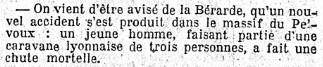
\includegraphics[height=1.7cm]{images/Le_Temps_1931-07-29_Herbrand-BnF.jpg}\vspace{1cm}

\tt
\begin{minipage}{13.5cm}\setstretch{0.8}\normalsize
Wir haben soeben aus La Bérarde erfahren, dass sich ein neuer Unfall auf dem Pelvoux ereignet hat:
ein junger Mann, der Mitglied einer dreiköpfigen Gruppe aus Lyon gewesen ist, stürzte zu Tode.
\end{minipage}

% 
% We have just learned from Le Bérarde that a new accident has occurred on the Pelvoux plateau: a young man, part of a three-man company from Lyons, has fallen to his death.
\bigskip\normalsize

~\hspace{\stretch{1}}-- Le Temps, Montag, 29. Juli 1931
\end{center}

\end{frame}
\egroup

\begin{frame}\frametitle{Resolution für Prädikatenlogik}

Ein konkreter Algorithmus zum logischen Schließen:
\begin{enumerate}[(1)]
\item \alert{Logische Konsequenz auf Unerfüllbarkeit reduzieren}
\item \alert{Formeln in Klauselform umwandeln}
	\begin{itemize}
	\item Formel bereinigen
	\item Negationsnormalform bilden
	\item Pränexform bilden
	\item Skolemform bilden
	\item Konjunktive Normalform bilden
	\end{itemize}
\item \alert{Resolutionsverfahren anwenden}
	\begin{itemize}
	\item Unifikation zum Finden passender Klauseln
	\item \textcolor{devilscss}{Bilden von Resolventen bis zur Terminierung}
	\end{itemize}
\end{enumerate}

\end{frame}

\begin{frame}\frametitle{Unifikation}

\anybox{strongyellow}{
\redalert{Unifikationsalgorithmus}\\[1ex]
\emph{Eingabe:} Unifikationsproblem $G$\\
\emph{Ausgabe:} allgemeinster Unifikator für $G$, oder "`nicht unifizierbar"'\\[1ex]
%
Wende die folgenden Umformungsregeln auf $G$ an, bis keine Regel mehr zu einer Änderung führt:
\begin{itemize}
\item \alert{Löschen:} $\{t\unieq t\}\cup G' \leadsto G'$
\item \alert{Zerlegung:} $\{f(s_1,\ldots,s_n)\unieq f(u_1,\ldots,u_n)\}\cup G' \leadsto \{s_1\unieq u_1,\ldots,s_n\unieq u_n\}\cup G'$
\item \alert{Orientierung:} $\{t\unieq x\}\cup G' \leadsto \{x\unieq t\}\cup G'$ falls $x\in\Slang{V}$ und $t\notin\Slang{V}$
\item \alert{Eliminierung:} $\{x\unieq t\}\cup G' \leadsto \{x\unieq t\}\cup G'\{x\mapsto t\}$ falls $x\in\Slang{V}$ nicht in $t$ vorkommt 
\end{itemize}
Wenn $G$ dann in gelöster Form ist, dann gib $\sigma_G$ aus.\\
Andernfalls gib aus "`nicht unifizierbar"'.
}

\end{frame}


\begin{frame}\frametitle{Unifikation von Atomen}

\defbox{Ein \redalert{Unifikator} für eine Menge $\mathcal{A}=\{A_1,\ldots,A_n\}$ von prädikatenlogischen Atomen ist eine Substitution $\theta$ mit $A_1\theta=A_2\theta=\ldots=A_n\theta$.
}\pause

\emph{Beobachtungen:}
\begin{itemize}
\item Eine Menge von Atomen $\mathcal{A}$ ist nur dann unifizierbar, wenn alle Atome das gleiche Prädikat verwenden, d.h. wenn es ein $\ell$-stelliges Prädikatensymbol $p$ gibt, so dass $A_i=p(t_{i,1},\ldots,t_{i,\ell})$ für alle $i\in\{1,\ldots,n\}$.
\item Dann ist $\sigma$ genau dann ein Unifikator für $\mathcal{A}$ wenn
$\sigma$ Unifikator für das folgende Unifikationsproblem $G_{\mathcal{A}}$ ist: 
\[ \{ t_{1,1}\unieq t_{2,1},\ldots,t_{n-1,1}\unieq t_{n,1},\ldots,t_{1,\ell}\unieq t_{2,\ell},\ldots,t_{n-1,\ell}\unieq t_{n,\ell} \} \]
\item Insbesondere ist der allgemeinste Unifikator für $G_{\mathcal{A}}$ auch der allgemeinste Unifikator für $\mathcal{A}$
\end{itemize}

\end{frame}

\begin{frame}\frametitle{Die Resolutionsregel}

\defbox{Die \redalert{Resolvente} von zwei Klauseln der Form\\[1ex]
\narrowcentering{$K_1=\{A_1,\ldots,A_n,L_1,\ldots,L_k\}$ und $K_2=\{\neg A'_1,\ldots,\neg A'_m,L'_1,\ldots,L'_\ell\}$,}\\[1ex]
für welche $\sigma$ der allgemeinste Unifikator der Menge $\{A_1,\ldots,A_n,A'_1,\ldots,A'_m\}$
ist und $L_i,L'_j$ beliebige Literale sind, ist die Klausel
$\{L_1\sigma,\ldots,L_k\sigma,L'_1\sigma,\ldots,L'_\ell\sigma\}$.
}\medskip\pause

\examplebox{Beispiel: Die Klausel $K_1=\{\neg\textsf{Mensch}(x),\textsf{hatVater}(x,f(x))\}$ und die Klausel $K_2=\{\neg\textsf{hatVater}(z,v),\textsf{hatKind}(v,z)\}$ können resolviert werden. Ein allgemeinster Unifikator von $\{\textsf{hatVater}(x,f(x)),\textsf{hatVater}(z,v)\}$
ist $\sigma=\{z\mapsto x,v\mapsto f(x)\}$.
Die entsprechende Resolvente von $K_1$ und $K_2$ ist $\{\neg\textsf{Mensch}(x),\textsf{hatKind}(f(x),x)\}$.
}

\end{frame}

\begin{frame}\frametitle{Resolution: Beispiel (1)}
 
 Wir hatten die folgende Beispielformel $F$ betrachtet:
%  
 \begin{align*}
& \forall x.\big((W(x)\wedge\neg L(x))\vee (L(x)\wedge\neg W(x))\big) \\
{}\wedge{} & \big(\exists x.W(x)\to(\forall x.W(x) \vee \forall x.L(x))\big) \\
{}\wedge{} & \big(\exists x.L(x)\to\neg(\forall x.W(x) \vee \forall x.L(x))\big)
\end{align*}

(Jeder ist Typ W oder Typ L / Ist einer Typ W, dann gibt es hier nur einen Typ / Ist einer Typ L, dann gibt es hier nicht nur einen Typ)\medskip

\alert{Folgt aus $F$, dass alle Typ W sind?}\bigskip\pause

\emph{Vorgehen:}
\begin{itemize}
\item Formalisiere diese Frage: \alert{$F\models \forall z.W(z)$?}\pause
\item Reduktion auf Unerfüllbarkeit: \alert{Ist $F\wedge\neg\forall z.W(z)$ unerfüllbar?}\pause
\item Klauselform: $F$ haben wir bereits in Klauselform gebracht. Wir können direkt die \alert{Klauseln für $\neg\forall z.W(z)$} hinzufügen:
\begin{itemize}
\item Bereinigte NNF (und Pränexform): \alert{$\exists z.\neg W(z)$}
\item Skolemform (und KNF): \alert{$\neg W(a)$} ($a$ ist Skolemkonstante)
\end{itemize}
\end{itemize}

\end{frame}

\begin{frame}[t]\frametitle{Resolution: Beispiel (2)}

Zusammen mit der Klauselform für $F$ erhalten wir die Klauseln:
%
{\small%
\[\begin{array}{rll}
(1) & \{W(x_1), L(x_1)\}\\[-0.5ex]
(2) & \{\neg L(x_1), L(x_1)\}\\[-0.5ex]
(3) & \{W(x_1), \neg W(x_1)\}\\[-0.5ex]
(4) & \{\neg L(x_1), \neg W(x_1)\}\\[-0.5ex]
(5) & \{\neg W(x_2), W(x_3), L(x_4)\}\\[-0.5ex]
(6) & \{\neg L(x_5),\ghost{$\neg W(f_6(x_1,x_2,x_3,x_4,x_5))\}$}\\[-0.5ex]
(7) & \{\neg L(x_5),\ghost{$\neg L(f_7(x_1,x_2,x_3,x_4,x_5))\}$} \\[-0.5ex]
(8) & \{\neg W(a)\}\\[-0.5ex]\pause
(9) & \{L(a)\} & \alert{(1)+(8)~~ \{x_1\mapsto a\}}\\[-0.5ex]\pause
(10) & \{\neg L(f(x_1,x_2,x_3,x_4,a))\} & \alert{(9)+(7)~~ \{x_5\mapsto a\}}\\[-0.5ex]\pause
\end{array}
\]}\vspace{-3.5ex}


\redalert{Problem:}\hspace{-2mm}%
\begin{minipage}[t]{8.5cm}\footnotesize\vspace{-2ex}
\begin{itemize}
\item $\neg L(f(x_1,x_2,x_3,x_4,a))$ bedeutet "`es gibt Nicht-Lügner"' (bezeichnet mit Termen der Form $f(x_1,x_2,x_3,x_4,a)$)\\[-2ex]
\item Dies sollte z.B. mit (1) "`Jeder Nicht-Lügner ist Wahrheitssager"' resolvieren\\[-2ex]
\item Aber $\{\neg L(f(x_1,x_2,x_3,x_4,a)), L(x_1)\}$ hat keinen Unifikator
\end{itemize}
\end{minipage}

\end{frame}

\begin{frame}\frametitle{Varianten von Klauseln}

Wir wissen: $\forall x.(F\wedge G)\equiv (\forall x.F\wedge \forall x.G)$ 
\bigskip

In Klauselform kann man sich also die Allquantoren direkt vor jeder einzelnen Klausel denken:
{\small%
\[\begin{array}{rl}
(1) & \forall x_1.\{W(x_1), L(x_1)\}\\[-0.5ex]
(2) & \forall x_1.\{\neg L(x_1), L(x_1)\}\\[-0.5ex]
& \ldots\\
(10) & \forall x_1,x_2,x_3,x_4.\{\neg L(f(x_1,x_2,x_3,x_4,a))\}
\end{array}
\]}\vspace{-1.5ex}\pause

Daher darf man die Variablen jeder Klausel einheitlich umbenennen, unabhängig von jeder anderen Klausel, z.B.
\[ \{\neg L(f(x_1,x_2,x_3,x_4,a))\} \quad\leadsto\quad \{\neg L(f(x'_1,x'_2,x'_3,x'_4,a))\} \]
Klauseln, die durch eineindeutige Umbenennung von Variablen entstanden sind, nennt man \redalert{Varianten} (einer Klausel)\\[0.5ex]
\alert{$\leadsto$ Wir bilden bei der Resolution Varianten um Konflikte von Variablen zu vermeiden}

\end{frame}

\begin{frame}[t]\frametitle{Resolution: Beispiel (3)}

Mit einer Variante von Klausel (11) gelingt die Resolution:
%
{\small%
\[\begin{array}{rll}
(1) & \{W(x_1), L(x_1)\}\\[-0.5ex]
(2) & \{\neg L(x_1), L(x_1)\}\\[-0.5ex]
(3) & \{W(x_1), \neg W(x_1)\}\\[-0.5ex]
(4) & \{\neg L(x_1), \neg W(x_1)\}\\[-0.5ex]
(5) & \{\neg W(x_2), W(x_3), L(x_4)\}\\[-0.5ex]
(6) & \{\neg L(x_5),\ghost{$\neg W(f_6(x_1,x_2,x_3,x_4,x_5))\}$}\\[-0.5ex]
(7) & \{\neg L(x_5),\ghost{$\neg L(f_7(x_1,x_2,x_3,x_4,x_5))\}$} \\[-0.5ex]
(8) & \{\neg W(a)\}\\[-0.5ex]
(9) & \{L(a)\} & \alert{(1)+(8)~~ \{x_1\mapsto a\}}\\[-0.5ex]
(10) & \{\neg L(f(x'_1,x'_2,x'_3,x'_4,a))\} & \alert{(9)+(7)~~ \{x_5\mapsto a\}}\\[-0.5ex]\pause
(11) & \{W(f(x'_1,x'_2,x'_3,x'_4,a))\} & \alert{(1)+(10)~~ \{x_1\mapsto f(x'_1,x'_2,x'_3,x'_4,a)\}}\\[-0.5ex]\pause
(12) & \{W(x_3), L(x_4)\} & \alert{(11)+(5)~~ \{x_2\mapsto f(x'_1,x'_2,x'_3,x'_4,a)\}}\\[-0.5ex]\pause
(13) & \{L(x_4)\} & \alert{(12)+(8)~~ \{x_3\mapsto a\}}\\[-0.5ex]\pause
(14) & \{\} & \alert{(13)+(10)~~ \{x_4\mapsto f(x'_1,x'_2,x'_3,x'_4,a)\}}
\end{array}
\]}

\end{frame}

\begin{frame}\frametitle{Resolution: Beispiel (4)}

Wir haben durch Resolution die \redalert{leere Klausel} $\{\}$ abgeleitet
\bigskip

Die leere Klausel bezeichnen wir auch mit \redalert{$\bot$}:
\begin{itemize}
\item Sie steht für die leere Disjunktion,
\item d.h. für eine falsche (unerfüllbare) Behauptung
\end{itemize}\bigskip

$\leadsto$ Wir haben gezeigt, dass die Klauselmenge unerfüllbar ist

$\leadsto$ Die geprüfte logische Konsequenz $F\models \forall z.W(z)$ gilt

\end{frame}

% \begin{frame}\frametitle{Varianten von Klauseln}
% 
% Es kann störend sein, wenn unterschiedliche Klauseln die selben Variablen verwenden.
% \medskip
% 
% \emph{Beispiel:} Für $\forall x.(\textsf{Mensch}(x)\to\exists y.(\textsf{hatVater}(x,y)\wedge\textsf{Mensch}(y)))$ erhalten wir die Klauselform
% %
% \[ \{\{\neg \textsf{Mensch}(x),\textsf{hatVater}(x,f(x))\},\{\neg \textsf{Mensch}(x),\textsf{Mensch}(f(x))\}\} \]
% %
% Die Klauseln sind nicht resolvierbar, weil $\{\neg \textsf{Mensch}(x),\textsf{Mensch}(f(x))\}$ keinen Unifikator hat.
% \bigskip\pause
% 
% Da jede Klausel für sich eine allquantifizierte Formel kodiert ($\forall$ distribuiert über $\wedge$) darf man Variablen aber umbenennen. Wir können z.B. die folgende \redalert{Variante} der zweiten Klausel bilden:
% \[ \{\neg \textsf{Mensch}(y),\textsf{Mensch}(f(y))\} \]
% $\{\neg \textsf{Mensch}(x),\textsf{Mensch}(f(y))\}$ hat den einen Unifikator, so dass wir z.B. die folgende Resolvente erhalten:
% \[\{\neg \textsf{Mensch}(y),\textsf{hatVater}(f(y),f(f(y)))\}\]
% 
% \end{frame}

\begin{frame}\frametitle{Der Resolutionsalgorithmus}

% Wir erhalten also folgenden Algorithmus

\codebox{%\redalert{Resolutionsalgorithmus}\\[1ex]
\emph{Eingabe:} Formel $F$
\begin{itemize}
\item Wandle $F$ in Klauselform um $\leadsto$ Klauselmenge $\mathcal{K}_0$
\item Für alle $i\geq 0$:
\begin{itemize}
\item $\mathcal{K}_{i+1}\defeq\mathcal{K}_i$
\item Für alle Klauseln $K_1,K_2\in \mathcal{K}_i$:
\begin{itemize}
\item Bilde von $K_1$ und $K_2$ Varianten $K'_1$ und $K'_2$, welche keine Variablen gemeinsam haben
\item Bilde alle möglichen Resolventen von $K'_1$ und $K'_2$ und füge diese zu $\mathcal{K}_{i+1}$ hinzu
\end{itemize}
\item Falls $\bot\in\mathcal{K}_{i+1}$, dann terminiere und gib "`unerfüllbar"' aus
\item Falls $\mathcal{K}_{i}=\mathcal{K}_{i+1}$, dann terminiere und gib "`erfüllbar"' aus
\end{itemize}
\end{itemize}
}

\emph{Anmerkung 1:} $K_1=K_2$ ist erlaubt und manchmal notwendig\\
\emph{Anmerkung 2:} $K'_1=K_1$ und/oder $K'_2=K_2$ ist möglich, sofern die Varianten keine gemeinsamen Variablen haben

\end{frame}

\begin{frame}\frametitle{Korrektheit des Resolutionsalgorithmus (1)}

Wir wollen den folgenden Satz schrittweise beweisen:

\theobox{Resolutionssatz: Sei $F$ eine prädikatenlogische Formel und $\mathcal{K}_i$ ($i\geq 0$) die vom Resolutionsalgorithmus ermittelten Klauselmengen. Dann sind die folgenden Aussagen äquivalent:
\begin{itemize}
\item $F$ ist unerfüllbar
\item Es gibt ein $\ell\geq 0$ mit $\bot\in\mathcal{K}_\ell$
\end{itemize}}\pause

\emph{Beweis (Korrektheit):} Wir zeigen Korrektheit eines Resolutionsschrittes; dann folgt die Behauptung durch Induktion über die Schrittzahl. Wir unterscheiden Klauseln $K$ vom Satz
$\forall K$, für den sie stehen (=Disjunktion mit allquantifizierten Variablen).
\bigskip

Wir hatten bereits erkannt, dass Varianten von Klauseln deren logische Konsequenzen sind (in der Notation des Algorithmus: $\forall K_1\models \forall K'_1$ und $\forall K_2\models \forall K'_2$).\bigskip

Wir zeigen noch die Korrektheit des reinen Resolutionsschrittes.

\end{frame}

\begin{frame}\frametitle{Korrektheit des Resolutionsalgorithmus (2)}

\emph{Beweis (Korrektheit, Fortsetzung):} Gegeben:
\begin{itemize}
\item Klauseln $K_1=\{A_1,\ldots,A_n,L_1,\ldots,L_k\}$ und $K_2=\{\neg A'_1,\ldots,\neg A'_m,L'_1,\ldots,L'_\ell\}$
\item (allgemeinster) Unifikator $\sigma$ der Menge $\{A_1,\ldots,A_n,A'_1,\ldots,A'_m\}$
\item zugehörige Resolvente $K=\{L_1\sigma,\ldots,L_k\sigma,L'_1\sigma,\ldots, L'_\ell\sigma\}$\pause
\end{itemize}

Sei $\Inter$ eine beliebige Interpretation.
\begin{itemize}
\item Falls $\Inter\models\forall K_1\wedge\forall K_2$, dann gilt auch $\Inter\models\forall (K_1\sigma)\wedge\forall (K_2\sigma)$\\ (die Substitution konkretisiert eine Allaussage)\pause
\item Also gilt für alle Zuweisungen $\Zuweisung$:~~~ $\Inter,\Zuweisung\models(K_1\sigma)\wedge (K_2\sigma)$\pause
\item \emph{Fall 1:} $\Inter,\Zuweisung\models A_1\sigma$ ($=A_2\sigma=\ldots=A'_m\sigma)$.\\ Dann gilt $\Inter,\Zuweisung\models L'_1\sigma\vee\ldots\vee L'_\ell\sigma$, und damit $\Inter,\Zuweisung\models K$\pause
\item \emph{Fall 2:} $\Inter,\Zuweisung\not\models A_1\sigma$ ($=A_2\sigma=\ldots=A'_m\sigma)$.\\ Dann gilt $\Inter,\Zuweisung\models L_1\sigma\vee\ldots\vee L_k\sigma$, und damit $\Inter,\Zuweisung\models K$\pause
\item Also gilt $\Inter\models\forall K$.
\end{itemize}
Da $\Inter$ beliebig ist gilt also $\forall K_1\wedge\forall K_2\models \forall K$.\\
Das heißt, jede Resolvente ist logische Konsequenz der resolvierten Klauseln.

\end{frame}

\begin{frame}\frametitle{Vollständigkeit des Resolutionsalgorithmus}

\theobox{Resolutionssatz: Sei $F$ eine prädikatenlogische Formel und $\mathcal{K}_i$ ($i\geq 0$) die vom Resolutionsalgorithmus ermittelten Klauselmengen. Dann sind die folgenden Aussagen äquivalent:
\begin{itemize}
\item $F$ ist unerfüllbar
\item Es gibt ein $\ell\geq 0$ mit $\bot\in\mathcal{K}_\ell$
\end{itemize}}

Bisher gezeigt: Die zweite Aussage impliziert die erste (\alert{Korrektheit})\bigskip

\alert{Vollständigkeit} ist die Umkehrung
\begin{itemize}
\item Jeder Widerspruch wird irgendwann durch Resolution gefunden
\item Das ist nicht so offensichtlich -- wir müssen dazu etwas weiter ausholen \ldots
\end{itemize}

\end{frame}

\bgroup
\setbeamercolor{background canvas}{bg=black}

\begin{frame}[plain]\label{frame_temps_b}
\color{white}
\begin{center}
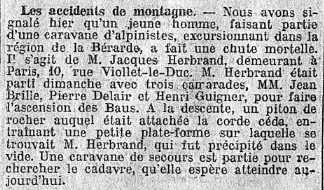
\includegraphics[height=4.5cm]{images/Le_Temps_1931-07-30_Herbrand-BnF.jpg}\bigskip

 \tt
\begin{minipage}{13.5cm}\setstretch{0.8}\normalsize
Wir hatten gestern erwähnt, dass ein junger Mann, der mit einer Gruppe von Bergsteigern in der Umgebung von La Bérarde unterwegs war, bei einem Sturz ums Leben kam.
Es handelte sich um M.~Jacques Herbrand, wohnhaft in der Rue Viollet-le-duc 10 in Paris. 
M.~Herbrand war am Sonntag mit drei Gefährten -- den Herren Jean Brille, Pierre Delair und Henri Guigner -- aufgebrochen, um Les Bans zu besteigen.
Beim Abstieg löste sich ein Kletterhaken, an dem das Seil befestigt war, und nahm eine kleine
Plattform mit sich, auf der sich M. Herbrand befand, welcher in den Abgrund stürzte.
Ein Bergungstrupp ist aufgebrochen um den Leichnam zu suchen und hofft ihn heute zu erreichen.
\end{minipage}

% 
% We mentioned yesterday that a young man, part of a company of Alpinists climbing in the area of Le Bérarde, fell to his death. he was M Jacques Herbrand, residing at 10 rue Viollet-le-duc, Paris. M Herbrand departed Sunday with three comrades, MM Jean Brille, Pierre Delair, and Henri Guigner, to ascend the Baus.\\[1ex]
% During the descent, the piton to which the line was attached gave way, carrying with it a small platform on which M Herbrand was situated, and fell into a chasm.\\[1ex]
% A rescue party has left to seek the body, which it hopes to reach today.
\bigskip

~\hspace{\stretch{1}}-- Le Temps, Dienstag, 30. Juli 1931
\end{center}
\end{frame}

\frame[plain]{\label{frame_herbrand}\begin{center}\color{white}
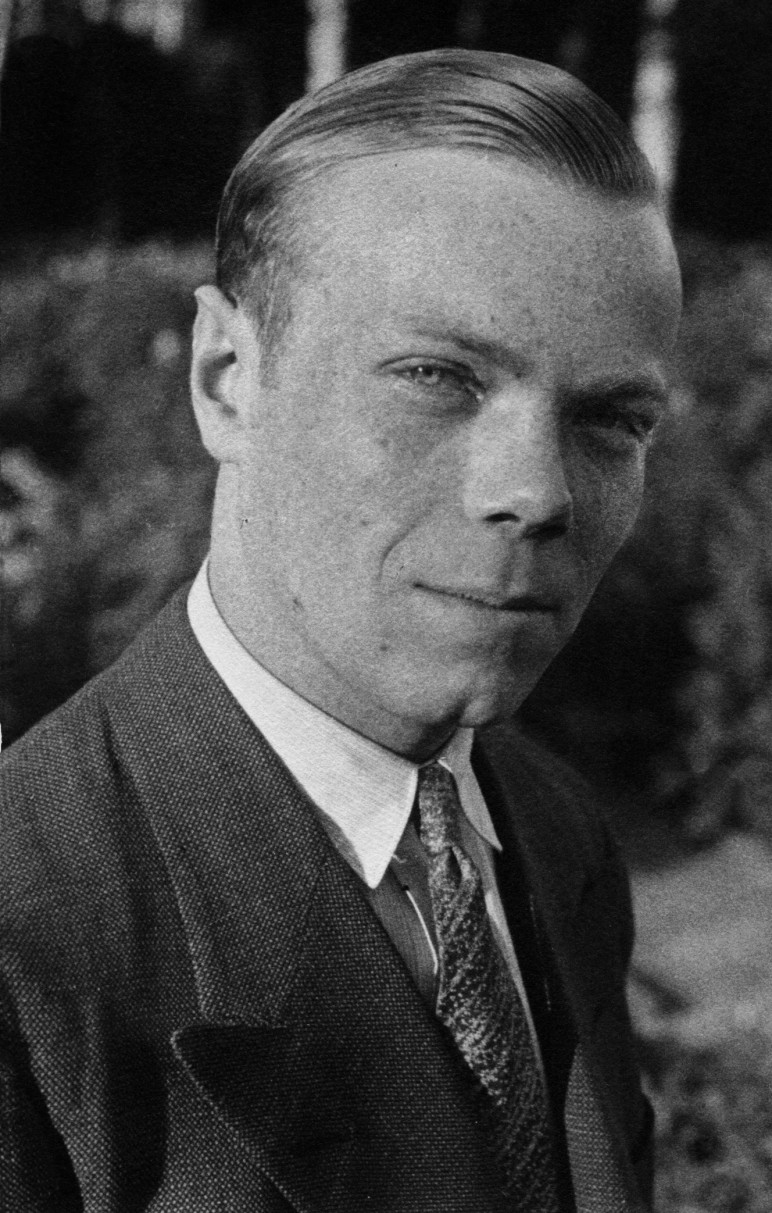
\includegraphics[height=6cm]{images/Herbrand.jpg}

\LARGE
Jacques Herbrand\medskip

\normalsize
\tt 12.2.1908 -- 27.7.1931
\end{center}}
\egroup

\begin{frame}\frametitle{Prädikatenlogische Modelle}

Wir wollen zeigen: Wenn es kein Modell für eine Formel gibt, dann leitet Resolution $\bot$ ab\bigskip

\alert{Problem:} Modelle sind sehr allgemeine Strukturen
\begin{itemize}
\item Beliebige Menge als Domäne
\item Systematische Betrachtung schwierig
\end{itemize}\bigskip\pause

\alert{Idee von Herbrand (und Skolem und Gödel)}:
\begin{center}
{\Large\redalert{"`Semantik aus Syntax"'}}\medskip

Konstruktion von Modellen direkt aus den Formeln, welche sie erfüllen sollen
\end{center}

\end{frame}

\begin{frame}\frametitle{Herbranduniversum}

Der Kern von Herbrands Idee ist eine "`syntaktische"' Domäne:\medskip

\defbox{Sei $a$ eine beliebige Konstante. Das \redalert{Herbranduniversum} $\Delta_F$ für eine Formel $F$ ist die
Menge aller variablenfreien Terme, die man mit Konstanten und Funktionssymbolen in $F$ und der zusätzlichen Konstante $a$ bilden kann:
\begin{itemize}
\item $a\in\Delta_F$
\item $c\in\Delta_F$ für jede Konstante aus $F$ 
\item $f(t_1,\ldots,t_n)\in\Delta_F$ für jedes $n$-stellige Funktionssymbol aus $F$ und alle Terme $t_1,\ldots,t_n\in\Delta_F$
\end{itemize}
}

\emph{Anmerkung:} Das Herbrand-Universum ist immer abzählbar, manchmal endlich und niemals leer.\pause

\examplebox{Beispiel: Für die Formel $F=p(f(x),y,g(z))$ ergibt sich das Herbranduniversum
$\Delta_F=\{a,f(a),g(a),f(f(a)),f(g(a)),g(f(a)),g(g(a)),\ldots\}$.
}

\end{frame}

\begin{frame}\frametitle{Herbrandinterpretationen}

Mit dem Herbrand-Universum als Domäne kann man Interpretationen definieren, die Terme "`durch sich selbst"' interpretieren:\medskip

\defbox{Eine \redalert{Herbrandinterpretation} für eine Formel $F$ ist eine Interpretation $\Inter$ für die gilt:
\begin{itemize}
\item $\Delta^\Inter=\Delta_F$ ist das Herbrand-Universum von $F$
\item Für jeden Term $t\in\Delta_F$ gilt $t^\Inter=t$
\end{itemize}
$\Inter$ ist ein \redalert{Herbrandmodell} für $F$ wenn zudem gilt $\Inter\models F$.}

\emph{Anmerkung:} Die Definition stellt Bedingungen an Grundbereich und Terminterpretation, aber sie lässt auch viele Freiheiten (z.B. die Interpretation von Prädikatensymbolen)

\end{frame}

\begin{frame}\frametitle{Beispiel}

Betrachten wir wieder die (skolemisierte) Formel $F=\forall x.\textsf{hatVater}(x,f(x))$.\bigskip

Herbranduniversum: $\Delta_F=\{a,f(a),f(f(a)),\ldots\}$\medskip

Alle Herbrandinterpretationen stimmen auf der Domäne und (dem relevanten Teil) der Terminterpretation überein.
\begin{itemize}
\item $\Inter_1$ mit $\textsf{hatVater}^{\Inter_1}=\emptyset$ ist kein Herbrandmodell
\item $\Inter_2$ mit $\textsf{hatVater}^{\Inter_2}=\{\tuple{t,f(t)}\mid t\in\Delta_F\}$ ist ein Herbrandmodell
\item $\Inter_3$ mit $\textsf{hatVater}^{\Inter_3}=\Delta_F\times\Delta_F$ ist ein Herbrandmodell
\end{itemize}

\end{frame}

\begin{frame}\frametitle{Syntax vs. Semantik}

Bei Herbrandinterpretationen kann man semantische Elemente (wie sie in Zuweisungen vorkommen) durch syntaktische Elemente (wie sie in Substitutionen vorkommen) ausdrücken:\medskip

\theobox{Lemma: Für jede Herbrandinterpretation $\Inter$, jede Zuweisung $\Zuweisung$ für $\Inter$, jeden Term $t\in\Delta^\Inter$ und jede Formel $F$ gilt:
\[ \Inter,\Zuweisung\{x\mapsto t\} \models F \qquad \text{gdw.}\qquad \Inter,\Zuweisung \models F\{x\mapsto t\}\]}

(ohne Beweis; einfach)
\bigskip

{\color{devilscss}\footnotesize \emph{Anmerkung:} Man kann ein entsprechendes Resultat auch für Nicht-Herbrand-Interpretationen zeigen. Dann muss man einfach den Term auf der linken Seite durch $t^{\Inter,\Zuweisung}$ ersetzen.}

\end{frame}

\begin{frame}\frametitle{Erfüllbar + Skolem = Erfüllbarkeit bei Herbrand}

\theobox{Satz: Ein Satz $F$ in Skolemform ist genau dann erfüllbar, wenn $F$ ein
Herbrandmodell hat.}\pause

\emph{Beweis:} $(\Leftarrow)$ ist klar, da Herbrandmodelle auch Modelle sind.\bigskip\pause

$(\Rightarrow)$ Sei $\Inter\models F$ ein Modell für $F$. Wir definieren eine Herbrandinterpretation $\Jnter$ indem wir festlegen:
\begin{itemize}
\item $p^\Jnter=\{\tuple{t_1,\ldots,t_n}\mid\tuple{t_1^\Inter,\ldots,t_n^\Inter}\in p^\Inter\}$\\
{\footnotesize Anm.: $t_i$ sind variablenfrei, daher ist $t_i^\Inter$ wohldefiniert}
\end{itemize}
Behauptung: \alert{$\Jnter$ ist ein Herbrandmodell von $F$}

\end{frame}

\begin{frame}\frametitle{Beweis (Fortsetzung)}

\emph{Behauptung:} \alert{$\Jnter$ ist ein Herbrandmodell von $F$}\bigskip

$F$ hat die Form $\forall x_1,\ldots, x_n.G$, wobei $G$ quantorenfrei ist.\pause
\begin{itemize}
\item Aus $\Inter\models F$ folgt also $\Inter,\Zuweisung\models G$ für jede Zuweisung $\Zuweisung$ für $\Inter$\pause
\item Speziell gilt also für alle $t_1,\ldots,t_n\in\Delta_F$: $\Inter,\{x_1\mapsto t_1^{\Inter},\ldots,x_n\mapsto t_n^{\Inter}\}\models G$\pause
\item Daraus folgt: $\Inter\models G\{x_1\mapsto t_1,\ldots,x_n\mapsto t_n\}$  (analog zu Lemma)\pause
\item Daraus folgt: $\Jnter\models G\{x_1\mapsto t_1,\ldots,x_n\mapsto t_n\}$\\
{\footnotesize(Für Atome $G$ direkt aus Definition; die Aussage kann leicht auf größere Boolsche Verknüpfungen von Atomen verallgemeinert werden -- formal durch strukturelle Induktion)}\pause
\item Es folgt: $\Jnter,\{x_1\mapsto t_1,\ldots,x_n\mapsto t_n\}\models G$ (Lemma)
\end{itemize}
Der Schluss gilt für alle $t_1,\ldots,t_n\in\Delta_F$, d.h. $\Jnter\models F$.\qed

\end{frame}

\begin{frame}\frametitle{Gegenbeispiel}

Der Satz gilt nicht unbedingt, wenn Formeln nicht in Skolemform \ghost{sind:}\bigskip

\examplebox{Beispiel: Die folgende Formel ist offensichtlich erfüllbar:
\[ \exists x.p(x)\wedge\exists y.\neg p(y)\]
Die Formel verwendet aber keine Funktionen oder Konstanten\\
$\leadsto$ das Herbrand-Universum ist $\{a\}$
\bigskip

Aber keine Interpretation $\Inter$ mit Domäne $\{a\}$ ist Modell der Formel, da in diesem Fall entweder $p^\Inter=\emptyset$ oder $(\neg p)^\Inter=\emptyset$ ist.
}

Zum Vergleich die Skolemform der Formel dieses Beispiels:
\[ p(c)\wedge\neg p(d)\]
Hier gibt es zwei (Skolem-)Konstanten im Herbrand-Universum\\
$\leadsto$ Es gibt ein Herbrand-Modell mit dieser Domäne

\end{frame}

% \begin{frame}\frametitle{Löwenheim-Skolem}
% 
% \theobox{Satz von Löwenheim${}^1$ und Skolem:
% Jede erfüllbare prädikatenlogische Formel hat ein abzählbares Modell (d.h. eines mit abzählbarer Domäne).}
% 
% \visible<3->{
% \emph{Beweis:} 
% \begin{itemize}
% \item Jede Formel $F$ kann in erfüllbarkeitsäquivalente Skolemform $F'$ überführt werden
% \item 
% Ist $F$ erfüllbar, so hat $F'$ ein (abzählbares) Herbrandmodell
% \item
% Man kann aus den Beweisen der Erfüllbarkeitsäquivalenz erkennen: jedes Modell von $F'$ ist auch ein Modell für $F$\qed
% \end{itemize}}\bigskip
% 
% {\footnotesize ${}^1$ Leopold Löwenheim${}^2$ (1878--1957): deutscher Logiker; 1915 erster Beweis des obigen Satzes; 1916 Soldat im 1. Weltkrieg; 1934 von den Nazis zwangspensioniert und als Privatlehrer tätig\\
% \visible<2->{\footnotesize ${}^2$ "`Note: One of the best predictors of success in mathematical logic is having an umlaut in your name"' -- S. Aaronson, Quantum Computing since Democritus. Cambridge, 2013.}
% 
% }
% 
% \end{frame}
% 
% \begin{frame}\frametitle{Historische Anmerkungen}
% 
% \begin{itemize}
% \item Der eben gezeigte "`Löwenheim-Skolem-Satz"' ist eigentlich der \alert{nach unten gerichtete Satz von Löwenheim und Skolem} (Downward Löwenheim-Skolem Theorem)
% \item Der \alert{nach oben gerichtete Satz von Löwenheim und Skolem}  (Upward Löwenheim-Skolem Theorem) besagt, dass jede erfüllbare Formel auch in Modellen beliebig großer Kardinalität erfüllbar ist\pause
% \item Der Legende nach war Skolem die Verwendung seines Namens in diesem Kontext unangenehm:\bigskip
% 
% \begin{quote}\color{purple}
% "`I follow custom in calling Corollary 6.1.4 the upward Löwenheim-Skolem theorem. But in fact Skolem didn't even believe it, because he didn't believe in the existence of uncountable sets."'\\
% -- W. Hodges, Model theory, Cambridge 1993
% \end{quote}
% \end{itemize}
% 
% \end{frame}


% \begin{frame}\frametitle{Herbrand-Expansionen}
% 
% \defbox{Die \redalert{Herbrand-Expansion} $HE(F)$ einer Formel $F=\forall x_1,\ldots, x_n.G$ in Skolemform ist die Menge:
% \[ HE(F)\defeq\{ G\{x_1\mapsto t_1,\ldots,x_n\mapsto t_n\}\mid t_1,\ldots,t_n\in\Delta_F\}\]
% }
% 
% $HE(F)$ ist also die (möglicherweise unendliche) Menge von \ghost{variablen-}\\ freien Sätzen, die in Herbrandmodellen von $F$ gelten müssten.
% \pause\bigskip
% 
% \redalert{Quantorenfreie Sätze = aussagenlogische Formeln:}
% \begin{itemize}
% \item $HE(F)$ enthält Formeln ohne Variablen, d.h. Boolsche Kombinationen geschlossener Atome
% \item Geschlossene Atome können unabhängig voneinander wahr oder falsch sein, egal wie ihre genaue Struktur aussieht
% \item Wir können sie also als "`ungewöhnlich benannte"' aussagenlogische Atome auffassen und die gesamte Formel aussagenlogisch interpretieren
% \end{itemize}
% \alert{$\leadsto$ $HE(F)$ als aussagenlogische Theorie}
% 
% 
% \end{frame}
% 
% \begin{frame}\frametitle{Gödel, Herbrand, Skolem}
% 
% \theobox{Satz von Gödel, Herbrand \& Skolem: Eine Formel $F$ in Skolemform ist genau dann erfüllbar, wenn $HE(F)$ aussagenlogisch erfüllbar ist.}\pause
% 
% \emph{Beweis:} Wir zeigen, dass $F=\forall x_1,\ldots,x_n.G$ genau dann ein Herbrandmodell hat, wenn $HE(F)$ aussagenlogisch erfüllbar ist:\pause
% 
% \begin{itemize}
% \item $\Inter$ ist ein Herbrandmodell von $F$\pause
% \item gdw. $\Inter,\{x_1\mapsto t_1,\ldots,x_n\mapsto t_n\}\models G$ für alle $t_1,\ldots,t_n\in\Delta_F$\pause
% \item gdw. $\Inter\models G\{x_1\mapsto t_1,\ldots,x_n\mapsto t_n\}$ für alle $t_1,\ldots,t_n\in\Delta_F$ (Lemma)\pause
% \item gdw. für alle $H\in HE(F)$ gilt $\Inter\models H$\pause
% \item gdw. $\Inter$ als aussagenlogisches Modell für $HE(F)$ angesehen werden kann.\qed
% \end{itemize}
% 
% \end{frame}
% 
% \begin{frame}\frametitle{Herbrand}
% 
% Als Korollar der gezeigten Ergebnisse erhalten wir ein wichtiges Resultat:
% 
% \theobox{Satz: Eine Formel $F$ in Skolemform ist genau dann unerfüllbar, wenn
% eine endliche Teilmenge von $E(F)$ aussagenlogisch unerfüllbar ist.}
% 
% \pause\emph{Beweis:} Das Kontrapositiv des Satzes von Gödel, Herbrand \& Skolem besagt:\medskip
% 
% Eine Formel $F$ in Skolemform ist genau dann unerfüllbar, wenn $HE(F)$ aussagenlogisch unerfüllbar ist.\bigskip
% 
% Der Satz folgt nun, weil jede unerfüllbare aussagenlogische Formelmenge eine endliche
% Teilmenge hat, die unerfüllbar ist (Kompaktheit der Aussagenlogik, siehe Formale Systeme, WS 2016/2017, Vorlesung 24)\qed
% 
% \end{frame}
% 
% \begin{frame}\frametitle{Prädikatenlogik semi-entscheiden}
% 
% Das Ergebnis Herbrands ermöglicht bereits einen naiven Algorithmus zur Semi-Entscheidung von Unerfüllbarkeit in der Prädikatenlogik:\bigskip
% 
% \emph{Gegeben:} Eine Formel $F$
% \begin{itemize}
% \item Wandle $F$ in Skolemform $F'$ um
% \item Definiere eine Reihenfolge der Formeln in $HE(F')$: $F_1,F_2,F_3,\ldots$
% \item Für alle $i\geq 1$:
% 	\begin{itemize}
% 	\item Prüfe ob die endliche Menge $\{F_1,\ldots, F_i\}$ aussagenlogisch unerfüllbar ist
% 	\item Falls ja, dann gib "`unerfüllbar"' aus; andernfalls fahre fort
% 	\end{itemize}
% \end{itemize}
% 
% Offenbar ist das \redalert{kein praktischer Algorithmus}, aber er zeigt Semi-Entscheidbarkeit
% 
% \end{frame}
% 
% \sectionSlide{Vollständigkeit der Resolution}
% 
% \begin{frame}\frametitle{Ansatz}
% 
% \alert{Herbrands Satz liefert uns auch eine Strategie für die Vollständigkeit des Resolutionsalgorithmus}\bigskip
% 
% \emph{Wir wissen bereits:}
% \begin{itemize}
% \item Unerfüllbarkeit einer Klauselmenge zeigt sich in der Unerfüllbarkeit ihrer Herbrand-Expansion
% \item Die Unerfüllbarkeit der Herbrand-Expansion kann man mit aussagenlogischer Resolution beweisen
% \item Prädikatenlogische Resolution verallgemeinert aussagenlogische Resolution indem wir direkt mit Klauseln arbeiten, die noch Variablen enthalten
% \end{itemize}
% \emph{Frage:} Kann man alle Schlüsse, die man auf expandierten Formeln aussagenlogisch erzeugen kann, auch direkt prädikatenlogisch (mit Variablen) erhalten?
% 
% \end{frame}
% 
% \begin{frame}\frametitle{Lifting-Lemma}
% 
% Wir zeigen: Ja, jeder aussagenlogische Schluss (auf der Expansion) kann auf einen prädikatenlogischen Schluss (auf den Klauseln mit Variablen) "`angehoben"' werden\medskip
% 
% \theobox{Satz (Lifting-Lemma): Seien $K_1$ und $K_2$ prädikatenlogische Klauseln mit
% Grundinstanzen $K'_1=K_1\sigma$ und $K'_2=K_2\sigma$.${^1}$\bigskip
% 
% Wenn $R'$ eine (aussagenlogische) Resolvente von $K'_1$ und $K'_2$ ist, dann gibt es
% eine prädikatenlogische Resolvente $R$, welche $R'$ als Grundinstanz hat.
% }
% 
% 
% {\footnotesize ${^1}$ Die Verwendung der selben Substitution für $K'_1$ und $K'_2$ ist keine Einschränkung, da wir durch Variantenbildung sicherstellen können, dass $K_1$ und $K_2$ keine Variablen gemein haben.
% 
% }
% 
% \end{frame}
% 
% \begin{frame}\frametitle{Lifting-Lemma: Beweis}
% 
% \theobox{Satz (Lifting-Lemma): Seien $K_1$ und $K_2$ prädikatenlogische Klauseln mit
% Grundinstanzen $K'_1=K_1\sigma$ und $K'_2=K_2\sigma$.\smallskip
% 
% Wenn $R'$ eine (aussagenlogische) Resolvente von $K'_1$ und $K'_2$ ist, dann gibt es
% eine prädikatenlogische Resolvente $R$, welche $R'$ als Grundinstanz hat.
% }
% 
% \emph{Beweis:} Sei $A'\in K'_1$ das (geschlossene) Atom, über das resolviert wurde, d.h. $\neg A'\in K'_2$.\smallskip\pause
% 
% Sei $\mathcal{A}_1\defeq\{A\mid A\in K_1,\;A\sigma=A'\}$ und $\mathcal{A}_2\defeq\{A\mid \neg A\in K_2, A\sigma=A'\}$.\smallskip\pause
% 
% Dann ist $\sigma$ ein Unifikator für $\mathcal{A}_1\cup\mathcal{A}_2$.\\ Also hat $\mathcal{A}_1\cup\mathcal{A}_2$ einen allgemeinsten Unifikator $\theta$.\smallskip\pause
% 
% Sei $R$ die Resolvente von $K_1$ und $K_2$ bzgl. $\theta$.\smallskip\pause
% 
% Dann enthalten $R'$ und $R$ Instanzen der gleichen Literale:
% $R'=\{L_1\sigma,\ldots,L_n\sigma\}$ und $R=\{L_1\theta,\ldots,L_n\theta\}$\smallskip\pause
% 
% Da $\theta$ allgemeinster Unifikator ist gibt es $\lambda$ mit $\sigma=\theta\circ\lambda$
% und es gilt: $R\lambda=\{L_1\theta\lambda,\ldots,L_n\theta\lambda\}=\{L_1\sigma,\ldots,L_n\sigma\}=R'$\qed
% 
% 
% \end{frame}
% 
% 
% \begin{frame}[t]\frametitle{Vollständigkeit der Resolution (1)}
% 
% \theobox{Resolutionssatz: Sei $F$ eine prädikatenlogische Formel und $\mathcal{K}_i$ ($i\geq 0$) die vom Resolutionsalgorithmus ermittelten Klauselmengen. Dann sind die folgenden Aussagen äquivalent:
% \begin{itemize}
% \item $F$ ist unerfüllbar
% \item Es gibt ein $\ell\geq 0$ mit $\bot\in\mathcal{K}_\ell$
% \end{itemize}}\pause
% 
% \emph{Beweis (Vollständigkeit):} Sei $F$ unerfüllbar
% \begin{itemize}
% \item Dann ist $HE(F)$ unerfüllbar
% \item Dann gibt es eine (endliche) aussagenlogische Resolutionsableitung von $\bot$ aus $HE(F)$
% \item Die Ableitung erzeugt eine endliche Folge von Klauseln: $K_1',K_2',\ldots,K_{m-1}',K_m'=\bot$
% \item \alert{Behauptung:} Jede Klausel $K_i'$ ist Grundinstanz einer Klausel $K_i$ die in $\mathcal{K}_\ell$ vorkommt für ein $\ell\geq 0$.
% \end{itemize}
% 
% \end{frame}
% 
% \begin{frame}[t]\frametitle{Vollständigkeit der Resolution (2)}
% 
% % \theobox{Resolutionssatz: Sei $F$ eine prädikatenlogische Formel und $\mathcal{K}_i$ ($i\geq 0$) die vom Resolutionsalgorithmus ermittelten Klauselmengen. Dann sind die folgenden Aussagen äquivalent:
% % \begin{itemize}
% % \item $F$ ist unerfüllbar
% % \item Es gibt ein $\ell\geq 0$ mit $\bot\in\mathcal{K}_\ell$
% % \end{itemize}}
% 
% \emph{Beweis (Vollständigkeit):} \alert{Behauptung:} Jede Klausel $K_i'$ ist Grundinstanz einer Klausel $K_i$ die in $\mathcal{K}_\ell$ vorkommt für ein $\ell\geq 0$.
% \medskip\pause
% 
% Aussage klar für $K'_i\in HE(F)$: in diesem Fall ist $K'_i$ ist Grundinstanz einer Klausel $K_i$ in der Klauselform von $F$ und in $\mathcal{K}_0$\medskip\pause
% 
% Restlicher Beweis durch Induktion über $i$:
% \begin{itemize}
% \item Indukstionsannahme: Die Aussage gilt für alle $j<i$\pause
% \item $K'_i$ ist Resolvente zweier Klauseln $K'_a$ und $K'_b$ mit $a,b<i$\pause
% \item Laut Hypothese sind $K'_a$ und $K'_b$ also Instanzen von Klauseln $K_a$ und $K_b$ in einer Menge $\mathcal{K}_\ell$\pause
% \item Laut Lifting-Lemma ist demnach $K'_i$ ebenfalls die Instanz einer Klausel $K_i$, die durch Resolution aus $K_a$ und $K_b$ entsteht\pause
% \item Diese Resolvente ist also ebenfalls in einer Menge der Form $\mathcal{K}_{\ell'}$\qed
% \end{itemize}
% 
% 
% \end{frame}


\begin{frame}\frametitle{Zusammenfassung und Ausblick}

Die prädikatenlogische Resolution ist ein Semi-Entscheidungsverfahren für die Unerfüllbarkeit logischer Formeln\bigskip

Man kann Erfüllbarkeit auf Erfüllbarkeit über "`syntaktisch definierten"' Herbrandmodellen reduzieren
(Fortsetzung folgt)
% \bigskip
% 
% Prädikatenlogik kann verschiedene Unendlichkeiten nicht unterscheiden: Eine Theorie hat beliebig große unendliche Modelle genau dann wenn sie abzählbare Modelle hat

% In diesem Sinne ist Prädikatenlogik eine Kurzschreibweise für möglicherweise unendliche aussagenlogische Theorien
\bigskip

\anybox{yellow}{
Was erwartet uns als nächstes?
\begin{itemize}
\item Beweis der Vollständigkeit der Resolution
\item Logik über endlichen Modellen und ihre praktische Anwendung
\item Gödel
\end{itemize}
}

\end{frame}


\begin{frame}[t]\frametitle{Bildrechte}

Folie \ref{frame_temps_a}: Ausschnitt ``Le Temps'', 29. Juli 1931, gemeinfrei; Digitalisierung durch gallica.bnf.fr / Bibliothèque nationale de France; hier veröffentlicht unter CC-By-NC-SA~3.0
\medskip

Folie \ref{frame_temps_b}: Ausschnitt ``Le Temps'', 30. Juli 1931, gemeinfrei; Digitalisierung durch gallica.bnf.fr / Bibliothèque nationale de France; hier veröffentlicht unter CC-By-NC-SA~3.0
\medskip

Folie \ref{frame_herbrand}: Fotografie von Natasha Artin Brunswick, 1931, CC-By 3.0

\end{frame}


\end{document}
